\documentclass[a4paper, 12pt, UTF8]{article}

\usepackage[dvipsnames]{xcolor} % Code highlighting color
\usepackage[spanish]{babel} % Language 
\usepackage{indentfirst}
\usepackage{fontspec} 
\usepackage{fullpage}
\usepackage{csquotes}
\usepackage[a4paper, margin=2cm]{geometry} % To change the margins
\usepackage{graphicx} % Insert images
\usepackage[hidelinks]{hyperref} % Links color
\usepackage[final]{pdfpages}
\usepackage{ragged2e}
\usepackage{wrapfig} %To Text wrap
\usepackage{listings} % Add code
\usepackage{verbatim}
\usepackage[backend=bibtex,citestyle=ieee]{biblatex}
\usepackage{nameref}
\usepackage{tikz}
\usepackage{float}
\usepackage{subcaption}
\usepackage{url}
\usepackage{multirow}
\usepackage{colortbl}

\setlength{\parskip}{0.7em}
%\setlength{\parindent}{1cm}
\linespread{1.25}

\title{
	\Huge
	\textbf{Trabajo innovación} \\
	\scshape Uso de redes neuronales para la clasificación de células
	}
\author{
	Marc Asenjo i Ponce de León \and
	Joan Marcè i Igual \and
	Iñigo Moreno i Caireta
	}
\date{\today}

\addbibresource{Bibliografia.bib}


\begin{document}

\maketitle

\begin{figure}
	\centering
	
\includegraphics[width=\linewidth]{./simple_FIB}
\end{figure}

\newpage
\tableofcontents

\newpage

\section{Introducción}

En este trabajo nos hemos centrado en la investigación\cite{deepLearning} sobre distintos métodos de clasificación de células y como las redes neuronales pueden afectar a dichos métodos.

\section{Introducción al sistema de clasificación}

\subsection{Adquisición de datos}
El sistema que han ideado se basa en combinar tecnologías de fotometría e inteligencia artificial para clasificar correctamente una célula. El sistema tiene que ser capaz de analizar muchas células por segundo mientras pasan por un canal, de esta manera se podrán clasificar las células, aunque haya muchas pocas ocurrencias de una de las opciones, como pasa en el caso de la detección de células cancerígenas, donde la cantidad de células cancerígenas es mucho inferior a la de células en buen estado si la enfermedad aún no ha llegado a los estados más destructivos. Para ello han desarrollado un sistema innovador con el que consiguen capturar unos 36 millones de imágenes por segundo, con lo que se consigue una capacidad de analizar 100.000 células por segundo. Además permite que las células que viajan por el nanotubo se puedan desplazar a 10 metros por segundo.

\begin{figure}[H]
	\centering
	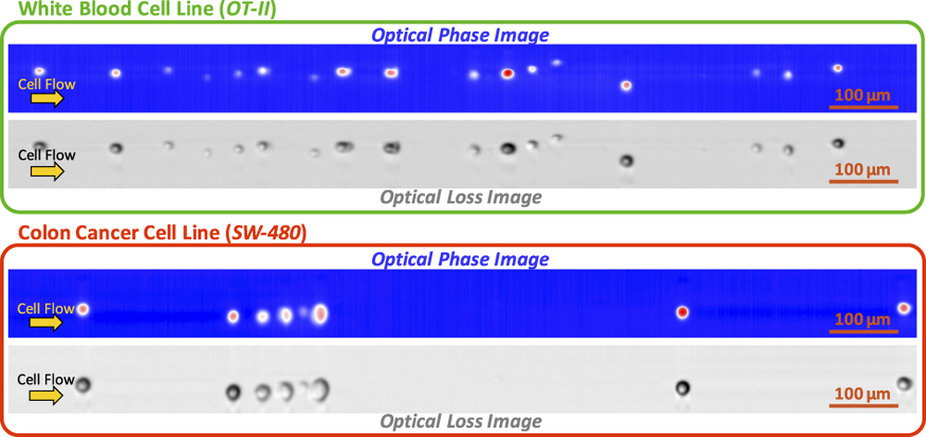
\includegraphics[width=0.95\textwidth]{Phase}
	\caption{Ejemplo de las fotos obtenidas por el sistema}
	\label{fig:phase}
\end{figure}

\subsection{Datos calculados}
El sistema es capaz de calcular muchos datos de cada célula, pero se pueden clasificar en dos grupos: los relacionados con la morfología de la célula y los que resultan de los análisis fotométricos. Entre los de la morfología de la célula se encuentran: el diámetro, el área, la circularidad de la célula, etc. El análisis fotométrico aporta datos como el índice de refracción de las células, su absorción y dispersión de luz, etc. Se puede encontrar una lista de todos los datos que utilizan en el informe científico. Como tienen tantos datos, muchos están relacionados entre ellos (ver \hyperref[fig:features]{figura~\ref{fig:features}}), haciendo un análisis de la correlación entre los datos, han encontrado que hay tres grupos muy relacionados: los datos relacionados con la morfología, los relacionados con la refracción, y los relacionados con la perdida y dispersión de la luz.

\begin{figure}[H]
	\centering
	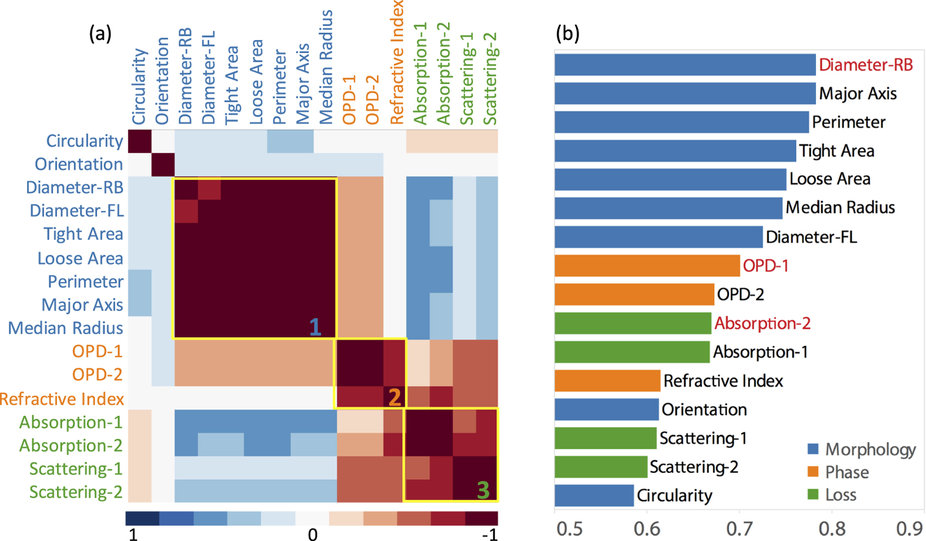
\includegraphics[width=0.95\textwidth]{features}
	\caption{(a) Correlación entre los diferentes datos calculados
		(b) Fiabilidad de cada uno de los paràmetros para hacer la clasificación}
	\label{fig:features}
\end{figure}

\section{Uso de tecnologías de inteligencia artificial}

Con toda esta gran cantidad de datos, se usa un algoritmo de redes neuronales para poder clasificar las células. El algoritmo de redes neuronales se basa en un árbol dirigido de nodos donde hay diferentes capas de nodos (ver \hyperref[fig:neural]{figura~\ref{fig:neural}}). Cada nodo hace una media ponderada de las salidas de los nodos de la capa anterior y después le aplica una función h a esta media para determinar la salida. La función h varía dependiendo de la capa, principalmente se usan dos funciones: la “función sigmoidea logística” es $h(a)=\frac{1}{1+e^{-a}}$ y la “unidad lineal rectificada” es $h(a)=max(0,a)$. Además, a cada capa se le añade un nodo que su salida siempre es uno. 
	
La última capa de nodos es la capa de decisión, en ella, cada nodo representa una de las posibles clasificaciones de la red. El algoritmo dirá que una célula pertenece a una clasificación dependiendo de un parámetro de aceptación.

\begin{figure}[h!]
	\centering
	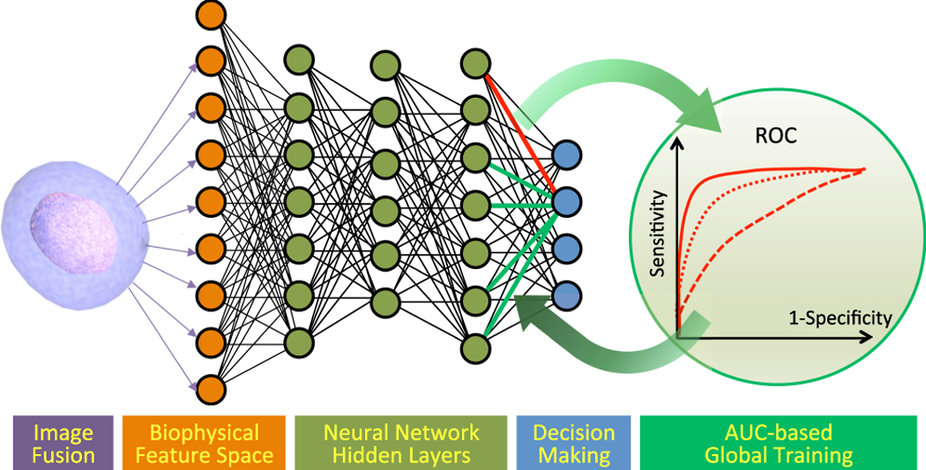
\includegraphics[width=0.95\textwidth]{neural}
	\caption{Esquema de la red neural}
	\label{fig:neural}
\end{figure}

Para encontrar los parámetros de la ponderación de las entradas de cada nodo se usa un método iterativo. Inicialmente, se asignan de manera aleatoria. En cada iteración se le pasa a la red neural una cantidad de ejemplos de los cuales se sabe el resultado esperado. Para cada uno de los nodos de la capa de decisión se calcula la curva ROC (del inglés Receiver Operating Characteristic). Esta curva es una representación de la sensibilidad (porcentaje de clasificación correcta cuando el resultado tendría que ser positivo) y especificidad (porcentaje de clasificación correcta cuando el resultado tendría que ser negativo). La curva se construye calculando la sensibilidad y especificidad para cada valor del parámetro de aceptación. Una vez hemos encontrado la curva ROC de cada nodo de la capa de decisión,  se ajustan los nodos de tal manera que el área que queda por debajo de cada curva ROC sea lo más alta posible.

\section{Impacto del descubrimiento}

Esta investigación permite hacer operaciones más profundas ya que normalmente el impacto que puede ocasionar la clasificación clásica puede generar que se activen o se inhiban ciertas señales, cambiando el comportamiento de ciertos tipos de células. Así pues este estudio permite sobrepasar estos problemas ya que no es necesario marcar las células para investigarlas y se puede hacer con una gran precisión y velocidad.

Como con este análisis se puede obtener más precisión, sensibilidad y seguridad, se está empezando a trabajar en la clasificación de células en busca de las que son potencialmente cancerígenas. En la \hyperref[fig:impacto_1]{Figura~\ref{fig:impacto_1}} se observa como este tipo de análisis permite obtener todo un conjunto de características para cada célula individualmente. 
Así pues, es relativamente fácil, a partir de ciertos parámetros, adivinar si hay células cancerígenas dentro del organismo y saber cuáles son.

\begin{figure}[H]
	\centering
	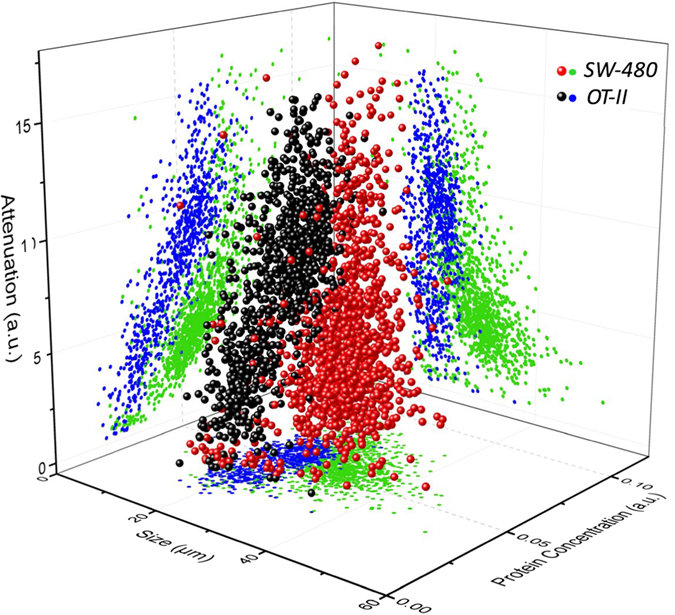
\includegraphics[width=0.95\textwidth]{impacto_1}
	\caption{Ejemplo de la clasificación de células cancerígenas donde se han ordenado en función de su tamaño, concentración de proteínas y atenuación}
	\label{fig:impacto_1}
\end{figure}

Otro ejemplo de uso son los biofueles generados a partir de microorganismos. Estos convierten el dióxido de carbono en lípidos que son mejores que los obtenidos por la agricultura tradicional. 

Actualmente, en todo el mundo se esta intentando mejorar la productividad de estos microorganismos y con este método podrán ser capaces de seleccionar directamente las micro algas que tienen un factor de crecimiento mayor y esto, es esencial en la industria de producción de biofuel para poder generar grandes cantidades de este producto y rebajar los costes. Se puede ver en la \hyperref[fig:impacto_2]{Figura \ref{fig:impacto_2}} como se han podido clasificar las diferentes algas en función de los contenidos de lípidos.

\begin{figure}[H]
	\centering
	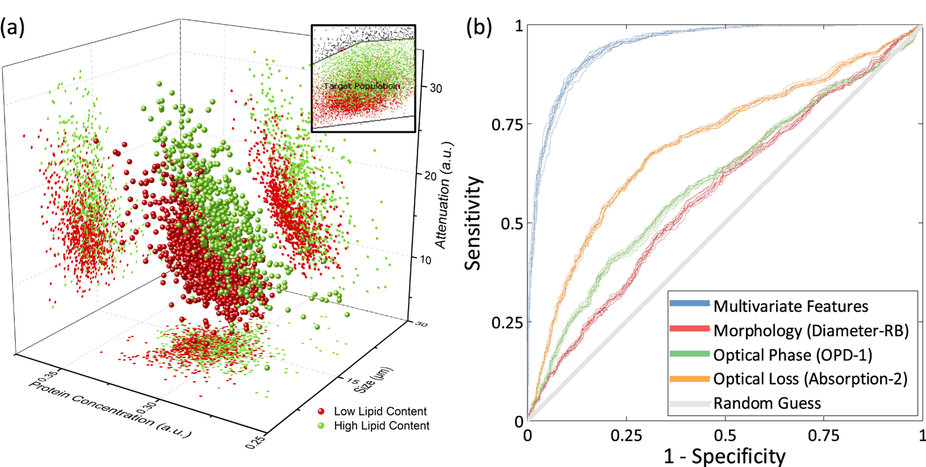
\includegraphics[width=\linewidth]{impacto_2}
	\caption{Ejemplo de la clasificación de micro algas, separando las que tienen un alto contenido de lípidos de las que tienen uno bajo}
	\label{fig:impacto_2}
\end{figure}

Así pues se puede ver que con este sistema se obtiene muchísima más precisión que con los métodos anteriores de manera que abre las puertas a un nuevo campo donde cada microorganismo se pueda clasificar individualmente. Se esta empezando a trabajar también en los microbots \cite{microbots} y quizá en un futuro se puedan emplear para clasificar todo aquello que no debería estar dentro de nuestro organismo como por ejemplo las bacterias o toda esa grasa innecesaria. 

\printbibliography

\end{document}